%!TEX root=../document.tex

\section{Plattform}

Um eine Anwendung zu Entwickeln, welche es erlaubt, Daten zu synchronisieren und eine Offline-Verfügbarkeit mittels einer lokalen Client-Datenbank zu Verfügung zu stellen, gibt es einige unterschiedliche Ansätze.
\\\\
Wie bereits im Unterricht besprochen bietet diff-sync eine einfache Möglichkeit mittels NodeJS Daten zu synchronisieren. Weiters gibt es unzählige Plattformen die solche Features anbieten, unter anderem Googles Firebase. Diese erlaubt es einfach, eine App zu Entwickeln, welche die Daten mit einer Firebase Datenbank synchronisieren. \cite{firebase}
\\\\
Schlussendlich wurde Couchbase als Plattform zur Umsetzung dieser Übung gewählt, da es mittels Sync Gateway und Couchbase Lite die umfangreichste und die meisten Funktion bietet. Ebenso unterstützt Couchbase sehr viele unterschiedliche Systeme und Programmiersprachen. Unter anderem auch C\# mit UWP, wobei die mit der UWP und .Net Plattform entwickelten Anwendungen mittels Xamarin auch auf Android und IOS laufen können. Da bereits einiges an Erfahrung mittels der Laborübung mit der UWP Plattform gesammelt worden ist, wurde für diese Aufgabe ebenfalls auf diese Plattform gesetzt.

\subsection{Couchbase}

Zur Umsetzung solch einer Anwendung mittels Couchbase werden 3 Komponenten benötigt.

\begin{itemize}
	\item \textbf{Couchbase Server}: Ein NoSQL Server, welcher zentral alle Daten verwaltet.
	\item \textbf{Sync Gateway}: Dies stellt die Schnittstelle zwischen den Server und den Clients dar. Sync Gateway bietet eine REST-Schnittstelle auf den Server zur Synchronisierung der Datensätze.
	\item \textbf{Couchbase Lite}: Stellt die Client Datenbank zu Verfügung. Kann offline verwendet werden, sobald eine Verbindung hergestellt werden kann, werden die Datensätze mittels Sync Gateway synchronisiert.
\end{itemize}

\begin{figure}[H]
	\centering
	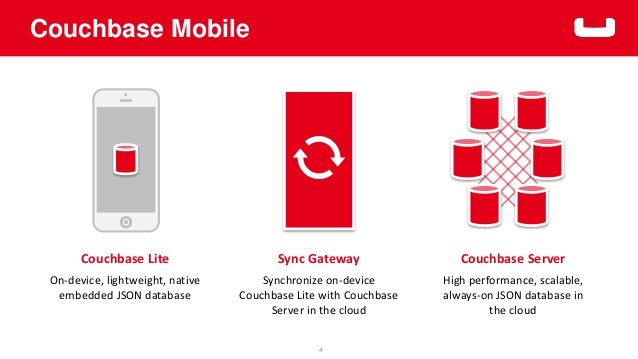
\includegraphics[width=0.9\linewidth]{img/building-net-apps-using-couchbase-lite-4-638}
	\caption{Umsetzung mittels Couchbase}
	\label{fig:building-net-apps-using-couchbase-lite-4-638}
\end{figure}

Einer der großen Vorteile dieser Plattform ist, dass der Client selber nie mit dem Server im Hintergrund kommuniziert bzw. umgesetzt werden muss. Die App selber greift nur auf die lokale Datenbank zu und nur diese Zugriffe müssen umgesetzt werden, die Synchronisierung übernimmt Sync Gateway und das Abspeichern der Couchbase Server. \cite{couchbaseapp}


\section{Umsetzung}

\subsection{Couchbase Server}

Zunächst wurde ein Couchbase Enterprise Server auf einen Server aufgesetzt, verwendet wurde die Version 5.1. Die Enterprise Software darf kostenlos zur Entwicklung und Testen verwendet werden, erst beim normalen Betrieb muss eine Lizenz erworben werden.
\\\\
Der Server mit der Datenbank ist unter der IP-Adresse 37.252.185.24 und dem Port 8091 erreichbar. Beim Aufsetzen wurde ein neuer Cluster erstellt und die RAM Zuweisung wurde verringert, ansonsten wurden alle Einstellung bei den default Werten belassen.
\\\\
Über diese Adresse kann nun auf das Admin Dashboard des Couchbase Servers zugegriffen werden. Über dieses wurde ein Benutzer \textit{UserEin} erstellt, welche volle Zugrissrechte auf den Bucket \textit{einkaufsliste} hat. \cite{couchbaseintro}

\subsection{Sync Gateway}

Wie auch der Couchbase wurde nun Sync Gateway auf dem Server installiert. Auch hier muss kaum etwas konfiguriert werden, nur beim erstmaligem Starten des Services muss eine Konfigurationsdatei angegeben werden.
\\\\
\begin{minted}{json}
	{
		"log": ["*"],
		"databases": {
			"db": {
				"server": "http://localhost:8091",
				"bucket": "einkaufsliste",
				"username": "UserEin",
				"password": "Einkaufsliste",
				"users": { "UserEin": { "disabled": false, "admin_channels": ["*"], "password": "Einkaufsliste" } },
				"sync": `function(doc) {
					channel("liste");
				}`
			}
		}
	}
	
\end{minted}

Diese JSON gibt den Namen der Datenbank an \textit{db}, weiters muss der Couchbase Server angegeben werden, dieser ist lokal aufrufbar. Nun wurde am Server ein Bucket mit dem Namen \textit{einkaufsliste} erstellt, dieser Name muss auch in der Konfiguration angegeben werden. Weiters muss der Benutzer sowie sein Passwort angegeben werden sein, sodass sich der Service mit den Server kommunizieren kann. Abschließend gibt eine \textit{sync} Funktion an, welche Dokumente synchronisiert werden sollen. Hierbei kann mittels Tags gearbeitet werden, sodass ein Client nur bestimmte Dokumente synchronisiert, in diesem Fall wurden alle Dokumente dem Channel \textit{liste} hinzugefügt.
\\\\
Ob alles richtig funktioniert hat, kann einerseits anhand der Meldung in der Konsole überprüft werden, anderseits muss die Adresse mit dem Port 4984, bei einer erfolgreichem Konfiguration folgendes zurückliefern. 

\begin{minted}{JSON}
	{"couchdb":"Welcome","vendor":{"name":"Couchbase Sync Gateway","version":"2.0"},"version":"Couchbase Sync Gateway/2.0.0(832;2d8a6c0)"}
\end{minted}

Wichtig zu beachten ist, sobald Sync Gateway aufgesetzt worden ist, sollte das Admin Dashboard des Couchbase Servers nicht mehr zum Verwalten der Dokumente verwendet werden, dies könnte nämlich zu Problemen bei der Synchronisierung zu den Clients führen. Sync Gateway bietet eine REST-Schnittstelle, über welche alle Dokumente im Bucket verwaltet werden können. \cite{syncgateway} 

\subsection{Couchbase Lite}

Wie bereits oben erwähnt wurde bei dieser Übung auf die UWP Plattform zurückgegriffen, da bei der letzten Übung bereits einiges an Erfahrung gesammelt worden ist und die Entwicklung sowie das Testen einfacher und schneller ist, da die Anwendung auch lokal getesten werden kann und nicht in einem Emulator oder auf einem Smartphone getesten werden muss.
\\\\
Um C
